\documentclass{article}

% if you need to pass options to natbib, use, e.g.:
% \PassOptionsToPackage{numbers, compress}{natbib}
% before loading nips_2017
%
% to avoid loading the natbib package, add option nonatbib:
% \usepackage[nonatbib]{nips_2017}

%\usepackage{nips_2017}

% to compile a camera-ready version, add the [final] option, e.g.:
\usepackage[final]{nips_2017}

\usepackage[utf8x]{inputenc} % allow utf-8 input
\usepackage[T2A]{fontenc}    % use 8-bit T1 fonts
\usepackage{hyperref}       % hyperlinks
\usepackage{url}            % simple URL typesetting
\usepackage{booktabs}       % professional-quality tables
\usepackage{amsfonts}       % blackboard math symbols
\usepackage{nicefrac}       % compact symbols for 1/2, etc.
\usepackage{microtype}      % microtypography
\usepackage[russian, english]{babel}
\usepackage{amsmath}
\usepackage{graphicx}
\usepackage{subcaption}
%\usepackage{subfigure}
%\usepackage{multicol}

\title{Optimal Portfolio Selection}

% The \author macro works with any number of authors. There are two
% commands used to separate the names and addresses of multiple
% authors: \And and \AND.
%
% Using \And between authors leaves it to LaTeX to determine where to
% break the lines. Using \AND forces a line break at that point. So,
% if LaTeX puts 3 of 4 authors names on the first line, and the last
% on the second line, try using \AND instead of \And before the third
% author name.

\author{
  Rasul~Khasianov \\
  SkolTech\\
  Moscow \\
  \texttt{Rasul.Khasianov@skoltech.ru} \\
  \And
  Oleg Gorodnitskii\\
  SkolTech\\
  Moscow\\
  \texttt{Oleg.gorodnitskii@skoltech.ru}
  \And
  Dmytro Fedoriaka\\
  SkolTech\\
  Moscow\\
  \texttt{Dmytro.Fedoriaka@skoltech.ru}\\
}

\begin{document}

\maketitle

\begin{abstract} 
This report details the working of our course project <<Optimal Portfolio Selection>>. We successfully studied the Markowitz theory and everything connected with it. We uploaded real data from sites, implemented several methods and compared them.
\end{abstract}

\section*{Links for materials (please, click on the name)}
\begin{enumerate}
\item \href{https://nbviewer.jupyter.org/github/fedimser/MarkowitzPortfolio/blob/master/code/Markovitz_new.ipynb}{Presentation}
\item \href{https://github.com/fedimser/MarkowitzPortfolio}{GitHub with code}
\end{enumerate}

\section*{Contribution}
\begin{enumerate}
\item[Dmytro] Initial problem statements and their solutions with CVXPY. Verification of solutions on real data.
\item[Oleg\;\;\;\;\;] Extraction and preparation of datasets (please see "Data" section). Consideration of different prediction techniques (trivial average prediction, polynomial interpolation, ARCH, GARCH, ARIMA) and ARIMA model adjustement.
\item[Rasul\;\;\;] Studying of the theory connected with sparse optimal portfolio, code implementing of this method and conducting numerical experiments. Writing report and making the presentation (structure, content, slides, plots).
\end{enumerate}

\section{Background}
The concepts of portfolio optimization and diversification have been instrumental in the development and understanding of financial markets and financial decision making. The major breakthrough came in 1952 with the publication of Harry Markowitz’s theory of portfolio selection (Markowitz et al.\ [1], 1952). The theory, popularly referred to as modern portfolio theory, provided an answer to the fundamental question: How should an investor allocate funds among the possible investment choices? Markowitz suggests that among the infinite number of portfolios that achieve a particular return objective, the investor should choose the portfolio that has the smallest variance. It was made possible by formulating the financial decision-making process as an optimization problem, so-called mean–variance optimization (MVO) problem.
\section{Problem formulation}
We consider an investment universe of $n$ assets $S_1, \dots S_n$ with uncertain future returns $R_1, \dots, R_n$. We denote by $R = [R_1, \dots, R_n]^T$ the vector of these returns. A portfolio is represented by the $n$-dimensional vector $ w= [w_1, \dots, w_n]^T$, where $w_i$ denotes the proportion of the total funds invested in security i. 

Suppose the return has a mean $\mu$ and a variance $\sigma^2$. What is the mean and standard deviation of the return $R$ of the portfolio? 
\[\mu(R) := \mathbb{E} [R] = \mathbb{E} \left[ \sum_{i=1}^n w_i R_i\right] =  \sum_{i=1}^n w_i \mathbb{E} [R_i] =  \sum_{i=1}^n w_i \mu_i\ = \vec{\mu}^T w\]
\begin{align*}
\sigma^2 (R) &= \mathbb{E}\left[(R - \mu)^2\right] = \mathbb{E}\left[\left(\sum_{i=1}^n w_i(R_i - \mu_i)\right)^2\right] = \\
&= \mathbb{E}\left[\sum_{i=1}^n \sum_{j=1}^n w_i w_j(R_i - \mu_i)(R_j - \mu_j)\right] =\\ 
&=\sum_{i=1}^n \sum_{j=1}^n \mathbb{E} \left[ w_i w_j(R_i - \mu_i)(R_j - \mu_j)\right] = \\
&=\sum_{i=1}^n \sum_{j=1}^n w_i w_j \mathrm{Cov} (R_i, R_j) = \sum_{i=1}^n \sum_{j=1}^n w_i w_j \sigma_{ij} =\\
&= w \Sigma w
\end{align*}
where $n\times n$ covariance matrix of the returns of all the assets is:
\begin{align*}
\Sigma = \begin{bmatrix}
\sigma_{11} & \sigma_{12} & \dots & \sigma_{1n}\\
\sigma_{21} & \sigma_{12} & \dots & \sigma_{1n}\\
\vdots & \vdots & \ddots & \vdots \\
\sigma_{n1} & \sigma_{n2} & \dots & \sigma_{nn}\\
\end{bmatrix}
\end{align*}
All valid covariance matrices are positive semidefinite matrices. Here we assume that $\Sigma$ satisfies the stronger property of positive definiteness. This is equivalent to assuming that none of the assets $S_1, S_2, \dots,S_n$ can be perfectly replicated by a combination of the remaining assets. Positive definiteness assumption ensures that $\Sigma$ is an invertible matrix. 

Using this notation, the MVO problem takes the form:
\begin{align}
\mathrm{minimize} &\;w \Sigma w \nonumber\\
\mathrm{s.t.} &\; \vec{\mu}^T w \geq p \label{eq:1}\\
&\; \sum_{i=1}^n w_i = 1 \nonumber
\end{align}
\section{Data}

Several sources of the data were considered. They can be listed in a following way:

\begin{enumerate}
\item Stock quotes downloaded from the "Yahoo!Finance" financial news site.\\

Considered tickers inlude stocks of large companies as "Apple" (quoted as "AAPL"), JP Morgan ("JPM") and AMD ("AMD").
\item Each 50-th symbol from the New York Stock Exchange publicly available data.\\
\item Each 10-th symbol from the New York Stock Exchange publicly available data. 
\end{enumerate}


20 tickers from "Yahoo!Finance" were used as a main source of data for experimental part of the project. Timeseries for all tickets needed to undergo a similar set of transformations (First difference and log-transformation) to make them stationary. All stocks timeseries had same ACF and PACF numbers after transformations, which allowed to fit ARIMA models with similar parameters to all of them.

\section{Models}
\subsection*{Model 1}
In the traditional Markowitz portfolio optimization, the objective is to find a portfolio which has minimal variance for a given expected return. This model $\ref{eq:1}$ was introduced above. 
\subsection*{Model 2}
Let the investor has some desired level of the risk $\sigma$. This means that the investor is ready to consider portfolios with a risk less than or equal to $\sigma$. At the same time, he wants to maximize expected return of the portfolio. We obtain the following optimization problem:
\begin{align}
\mathrm{minimize} &\; \vec{\mu}^T w \nonumber\\
\mathrm{s.t.} &\; w \Sigma w \leq \sigma \label{eq:2}\\
&\; \sum_{i=1}^n w_i = 1 \nonumber
\end{align}
\subsection*{Model 3}
Finally, we can assume that the investor is ready to take additional risks by increasing portfolio returns. That is, the optimal portfolio is the solution of the following optimization problem:
\begin{align}
\mathrm{minimize} &\; \vec{\mu}^T w - \lambda w \Sigma w \label{eq:3} \\
\mathrm{s.t.} &\;\sum_{i=1}^n w_i = 1 \nonumber
\end{align}
In this case, $\lambda$ represents the cost of risk in terms of profitability. When $\lambda$ is small, the penalization from entering more risky assets into the portfolio is small, which leads to the selection of more risky portfolios. When $\lambda$ is large, more conservative portfolios are selected.

All three problems are problems of quadratic programming. For this class of problems, there are effective computational algorithms. It is also worth noting that many popular additional constraints on the portfolio do not worsen the structure of the task. Here are some popular additional restrictions:
\begin{enumerate}
\item $w_i \geq 0 $ -- only long positions allowed;
\item $w_i \leq \alpha$ -- the share of each of the asset does not exceed a certain number $\alpha$.
\end{enumerate}
\subsection*{Model 4}
Markowitz Portfolio is usually dense (all components of $w$ are greater than zero), with many of its components close to zero. Such a portfolio structure is not always convenient for operations: it leads to relatively large commissions on the part of the broker. In this regard, it makes sense to consider the problem of solving a sparse optimal portfolio. 

Practical investing requires balancing portfolio optimality and simplicity. If investor has large set for investment opportunities then managing of all asset positions and transacting frequently is expensive and time-consuming.

The problem can be formulated as:
\[F = \frac{1}{2} w^T \Sigma w - w^T \mu + \lambda \|w\|_1\]
and it can be reformulated to the form of standard sparse regression loss functions:
$$F = \frac{1}{2} \left \|L^T  w - L^{-1} \mu \right\|_2^2 + \lambda  \| w\|_1$$
where $\Sigma = L L^T$ $-$ Cholesky decomposition
Indeed:
\begin{align*}
F &= \frac{1}{2} w^T \Sigma w - w^T \mu + \lambda \|w\|_1 \sim\\
& \sim \frac{1}{2} \left(w - \Sigma^{-1} \mu \right)^T \Sigma \left(w - \Sigma^{-1} \mu \right) + \lambda \|w\|_1 = \\
& = \frac{1}{2} \left(w - L^{-T} L^{-1} \mu \right)^T L L^{T}  \left(w - L^{-T} L^{-1}  \mu \right) + \lambda \|w\|_1 = \\
& = \frac{1}{2} \left[ L^T \left(w - L^{-T} L^{-1} \mu \right) \right]^T  \left[ L^T \left(w - L^{-T} L^{-1} \mu \right) \right]+ \lambda \|w\|_1 = \\
& = \frac{1}{2} \left \|L^T  w - L^{-1} \mu \right\|_2^2 + \lambda  \| w\|_1
\end{align*}
\section{Results}
The goal of our experimental evaluation was to investigate Markowitz theory in differrent cases. We conducted several experiments with described models and we obtained interesting results. 

Below we compare results for dense and sparse solutions, which have the largest differences.

\begin{figure}[!htb]
\centering
\caption{Results for simple formulations of this problem. (Left) The pie chart looks very dense. (Right) The profit has a high variance, which may increase the total risks.}
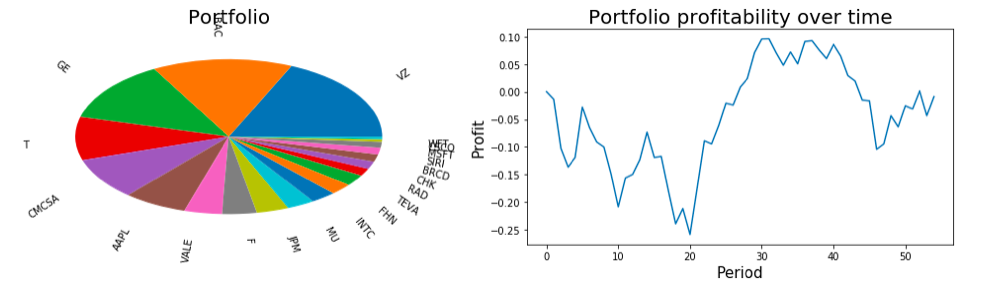
\includegraphics[width=1\textwidth]{image1.png}
\end{figure}

This figure the same for the first three models. Usually it gives about $2\%$ return. Here we predicted for 55 days in advance.

At the same time we have much better results for sparse solution:

\begin{figure}[!htb]
\centering
\caption{Results for sparse optimal formulation. (Left) The pie chart is really sparse. (Right) The profit has a low variance.}
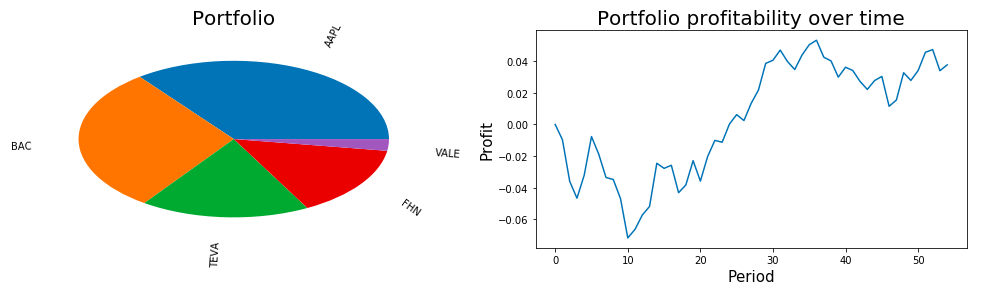
\includegraphics[width=1\textwidth]{image2.png}
\end{figure}

We see that regularization reflects the investor’s desire for portfolio simplicity. Intuitively, this penalty chooses the optimal weight vector by allocating a reasonable amount of wealth to a small subset of assets. 

Very intersting results we obtained for the model with regularization:

\begin{figure}[!htb]
\caption{Mean-Variance efficient portfolio}
\minipage{0.5\textwidth}
  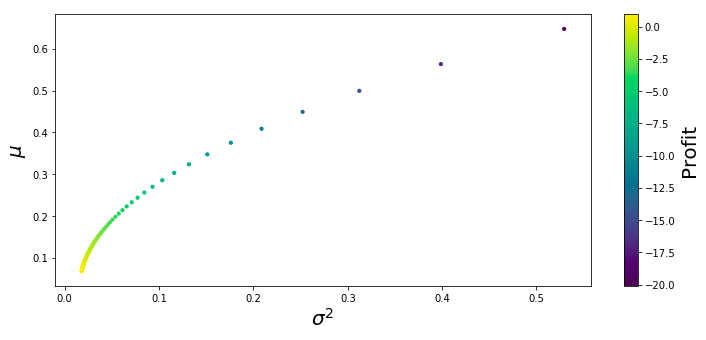
\includegraphics[width=\linewidth]{image3.png}
  \captionof*{figure}{Results withou regularization}
\endminipage\hfill
\minipage{0.5\textwidth}
  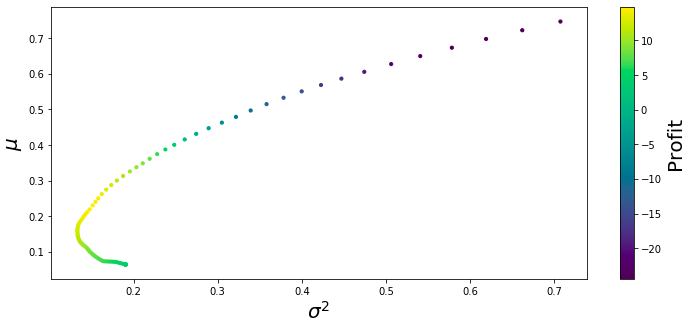
\includegraphics[width=\linewidth]{image4.png}
  \captionof*{figure}{Results with regularization}
\endminipage
\end{figure}
It is clear, that regularization is extended the set of optimal solutions! And we can find better results than for previous formulations of problem without regularization.

\section{Conclusion}
This paper has shown different approaches to mean-variance portfolio optimization from the investor’s perspective. We have described traditional formulations of this problem, that showed poor results and it we implemented an efficient algorithm for computing the optimal, sparse portfolios. This shows that adding an $l_1$ penalty to objective functions is a powerful tool for various portfolio construction tasks. 
\section*{References}
\small

[1] Markowitz, H (1952). Portfolio Selection. {\it Journal of Finance, 7}, pp.\ 77--91

[2] Puelz, D., Hahn, P. R. Carvalho, C. (2016). Sparse mean-variance portfolios: A penalized utility approach. {\it Submitted manuscript.}

% [2] Bower, J.M.\ \& Beeman, D.\ (1995) {\it The Book of GENESIS:
%   Exploring Realistic Neural Models with the GEneral NEural SImulation
%   System.}  New York: TELOS/Springer--Verlag.

% [3] Hasselmo, M.E., Schnell, E.\ \& Barkai, E.\ (1995) Dynamics of
% learning and recall at excitatory recurrent synapses and cholinergic
% modulation in rat hippocampal region CA3. {\it Journal of
%   Neuroscience} {\bf 15}(7):5249-5262.


\end{document}








